\block{Motivations}{
		\begin{minipage}{0.48\linewidth}
			\textbf{Current Objective :} Develop hybrid \textbf{\fcolorbox{color1!50}{color1}{finite element}} / \textbf{\fcolorbox{color1!50}{color1}{neural network}} methods.
		
			\vspace{-5pt}
			\hspace{495pt} \begin{minipage}{0.5\linewidth}
				\textbf{\textcolor{color2}{accurate}}
				\hspace{25pt}
				\textbf{\textcolor{color2}{quick + parameterized}}
			\end{minipage}
			
		\end{minipage}
		\begin{minipage}{0.48\linewidth}
			\centering
			\textbf{Problem considered :} $\qquad -\Delta u(x) = f(x) \quad \text{in } \Omega, \quad u(x) = g(x) \quad \text{on } \Gamma.$ \\
			Poisson problem with Dirichlet boundary conditions (BC).
		\end{minipage}
		
		\vspace{20pt}
		
		\begin{center}
			\begin{minipage}{0.48\linewidth}
				\centering
				\begin{tcolorbox}[
					colback=color1!50, % Couleur de fond de la boîte
					colframe=color2, % Couleur du cadre de la boîte
					arc=2mm, % Rayon de l'arrondi des coins
					boxrule=2pt, % Épaisseur du cadre de la boîte
					breakable, enhanced jigsaw,
					width=\linewidth
					]
					\textbf{OFFLINE}

					\vspace{-15pt}
				
					\begin{center}
						\begin{tikzpicture}
							\node at (0,3.5) {1 Geometry};
							\node[draw=none, inner sep=0pt] at (0,0) {
\includegraphics[width=6cm]{images/intro/objective_onegeom.pdf}};
							\node[color2,font=\Large] at (5,0.3) {+};
							\node at (13,2.6) {Several Forces};
							\node[draw=none, inner sep=0pt] at (13,0) {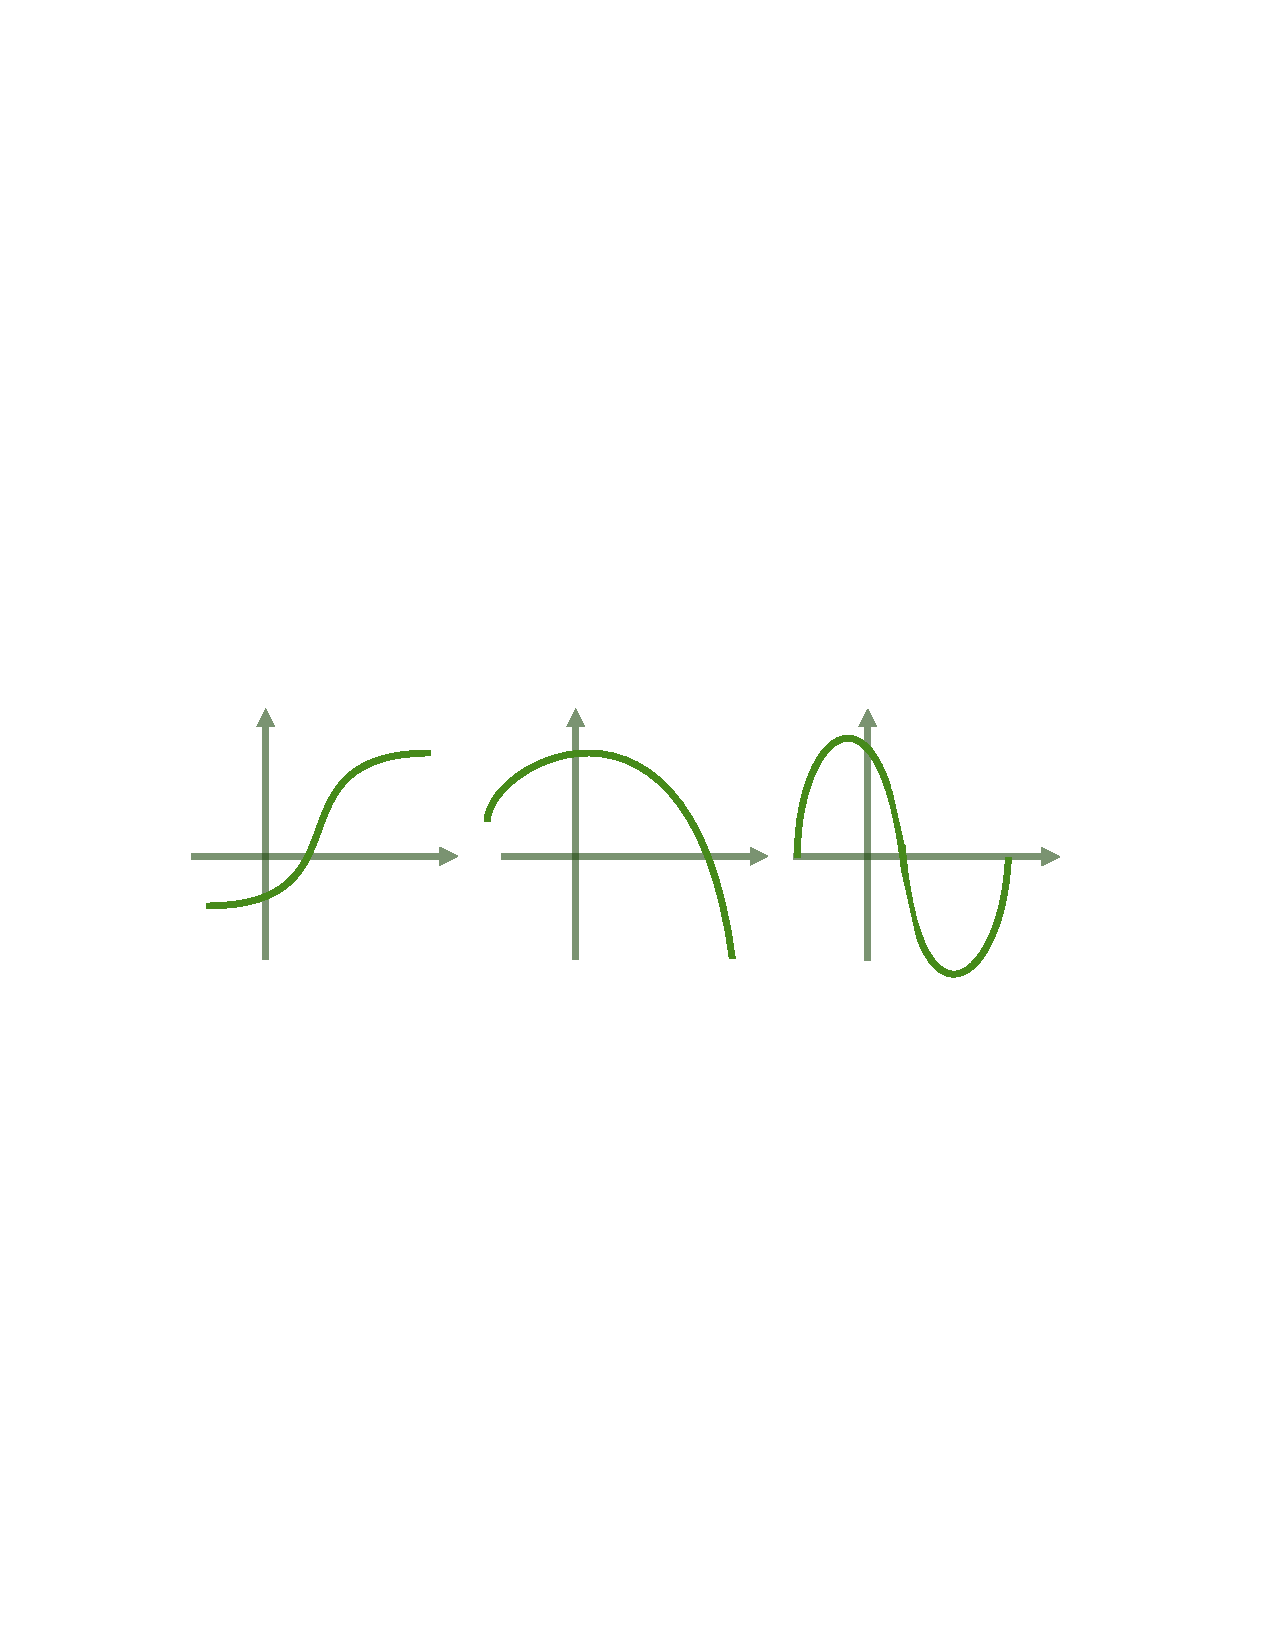
\includegraphics[width=12cm]{images/intro/objective_fct.pdf}};
							
							% Ajouter une flèche entre les deux rectangles
							\draw[->, color2, line width=4.5pt] (20.5,0.3) -- (23.5,0.3);
							%		
							\node[align=center] at (28,4) {Train a PINNs \\ \cite{raissi_physics-informed_2019}};
							\node[draw=none, inner sep=0pt] at (28,0) {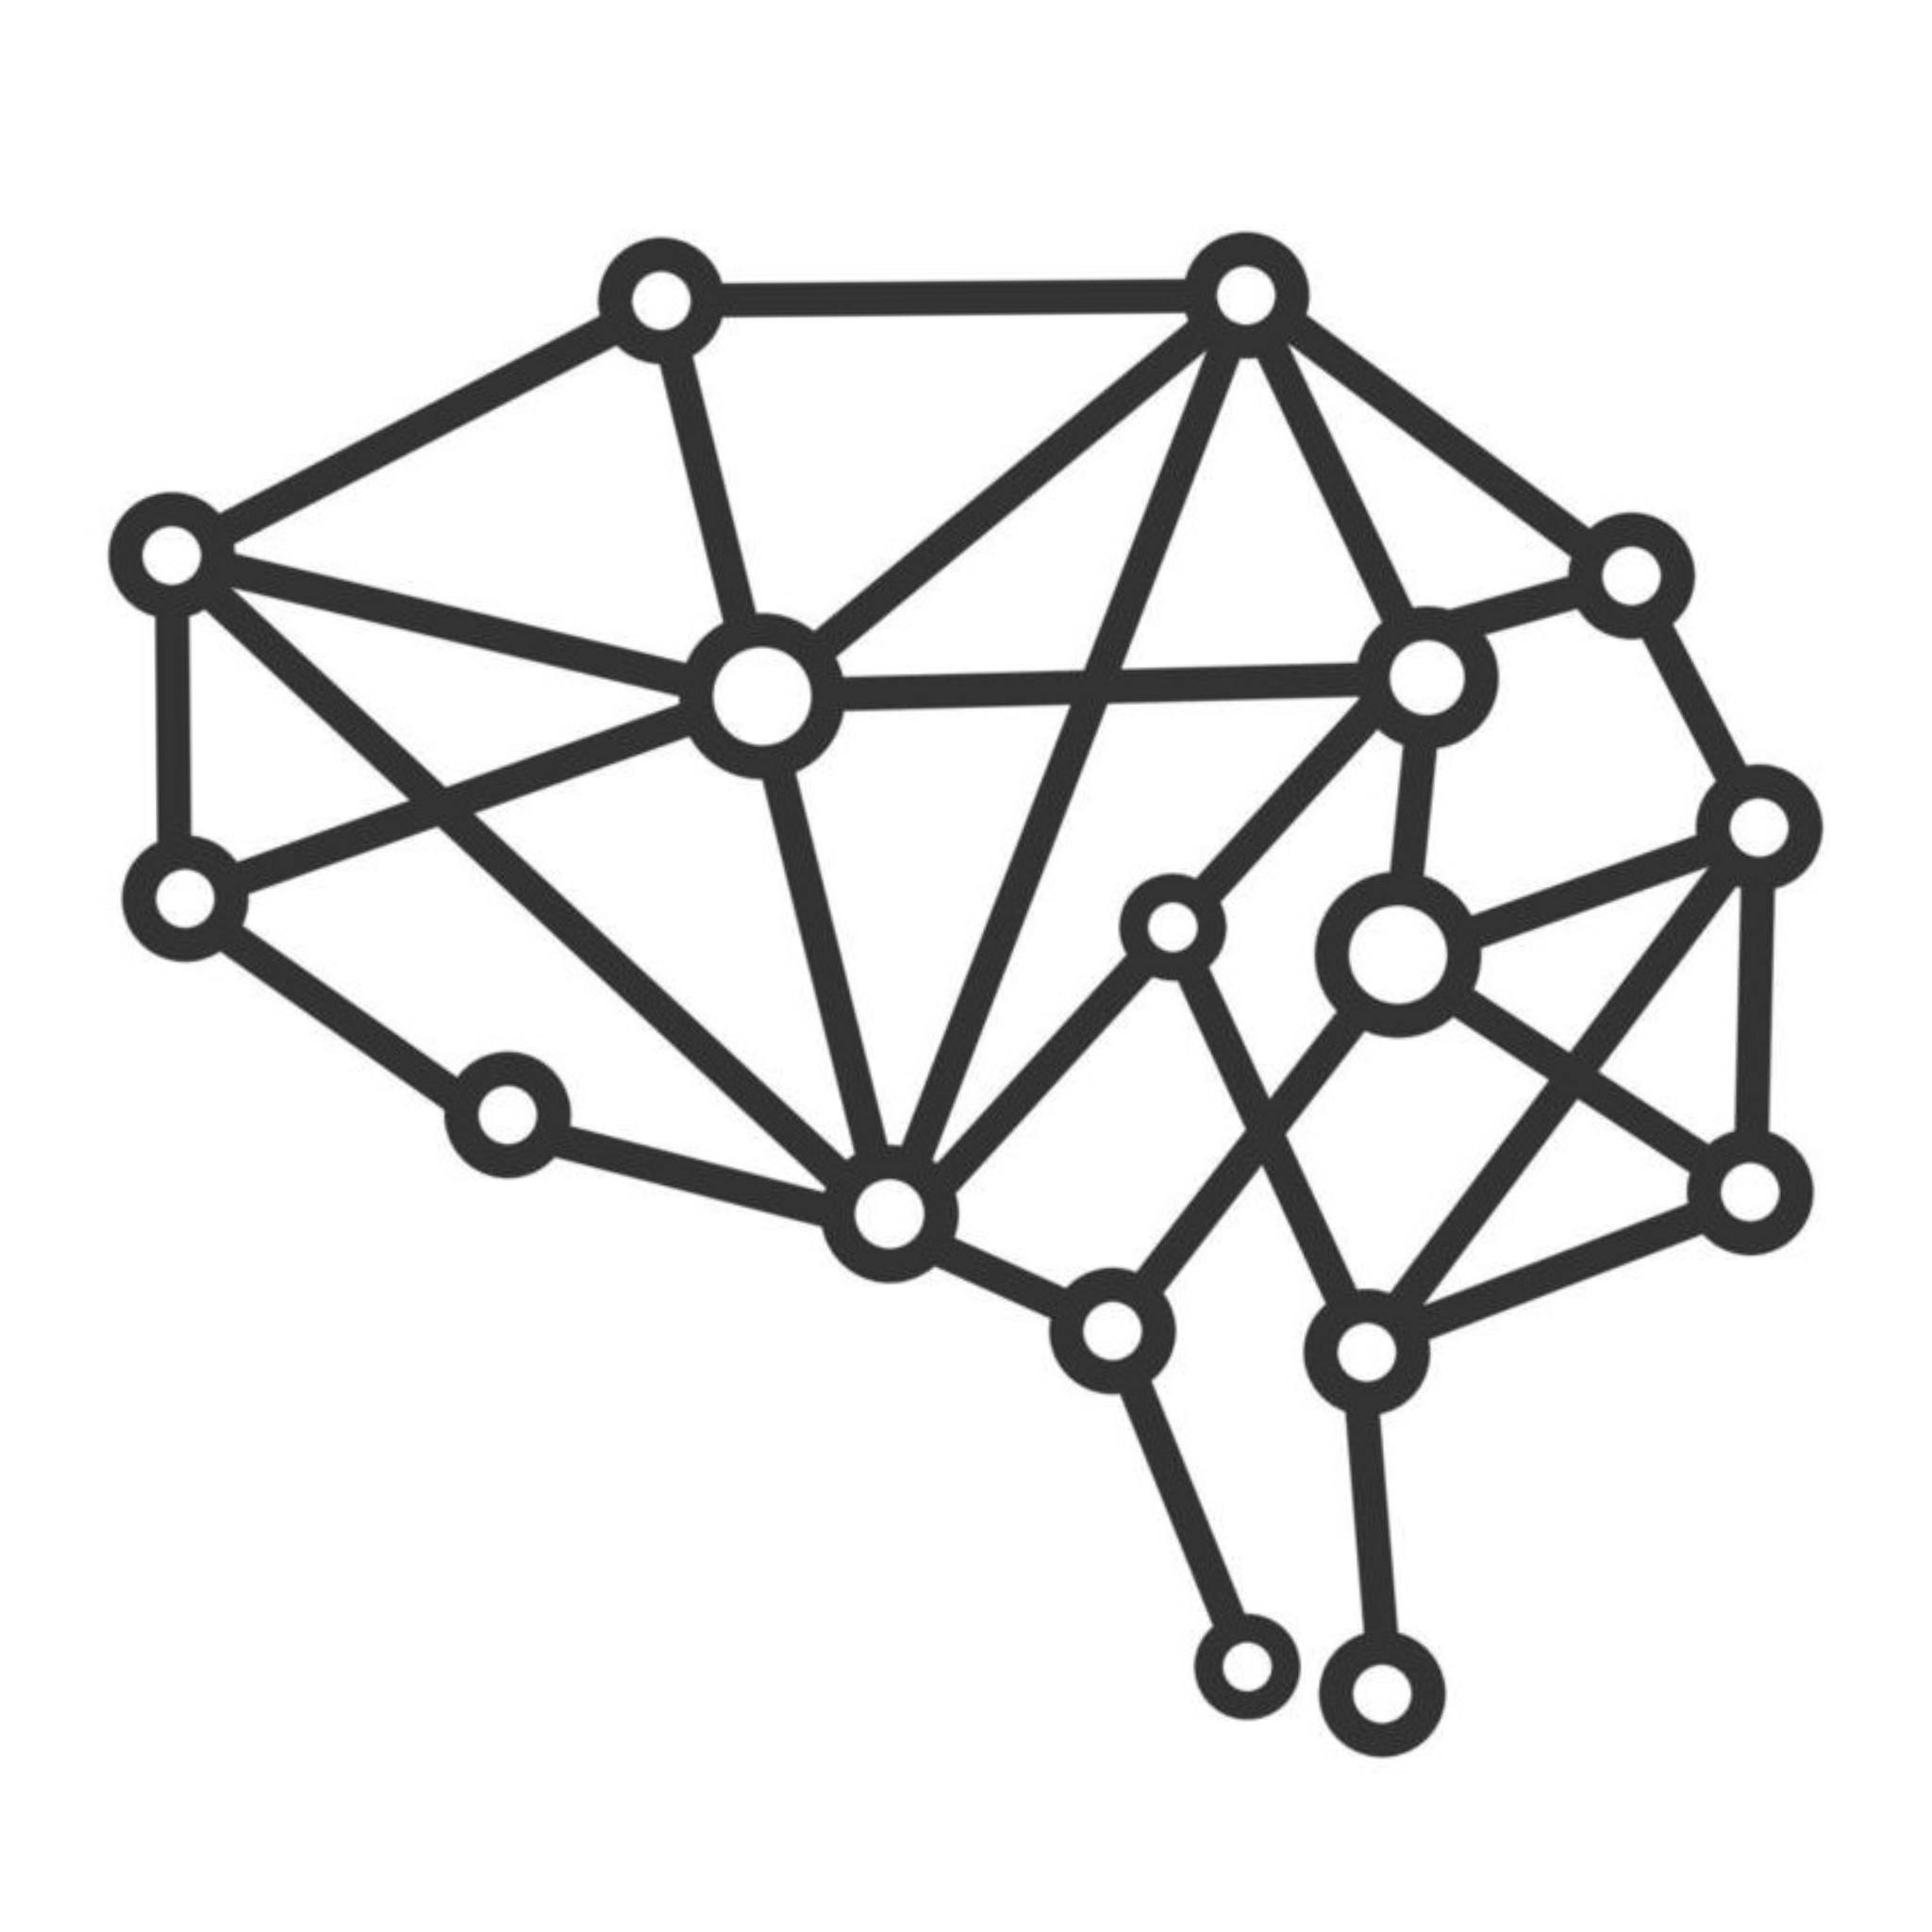
\includegraphics[width=6cm]{images/intro/objective_pinns.png}};				
						\end{tikzpicture}
					\end{center}
				\end{tcolorbox}
			\end{minipage}	
			\begin{minipage}{0.48\linewidth}
				\centering
				\begin{tcolorbox}[
					colback=color1!50, % Couleur de fond de la boîte
					colframe=color2, % Couleur du cadre de la boîte
					arc=2mm, % Rayon de l'arrondi des coins
					boxrule=2pt, % Épaisseur du cadre de la boîte
					breakable, enhanced jigsaw,
					width=\linewidth
					]
					\textbf{ONLINE}
					
					\vspace{-20pt}
					\begin{center}
						\begin{tikzpicture}
							\node at (0,2.6) {1 Geometry - 1 Force};
							\node[draw=none, inner sep=0pt] at (0,0) {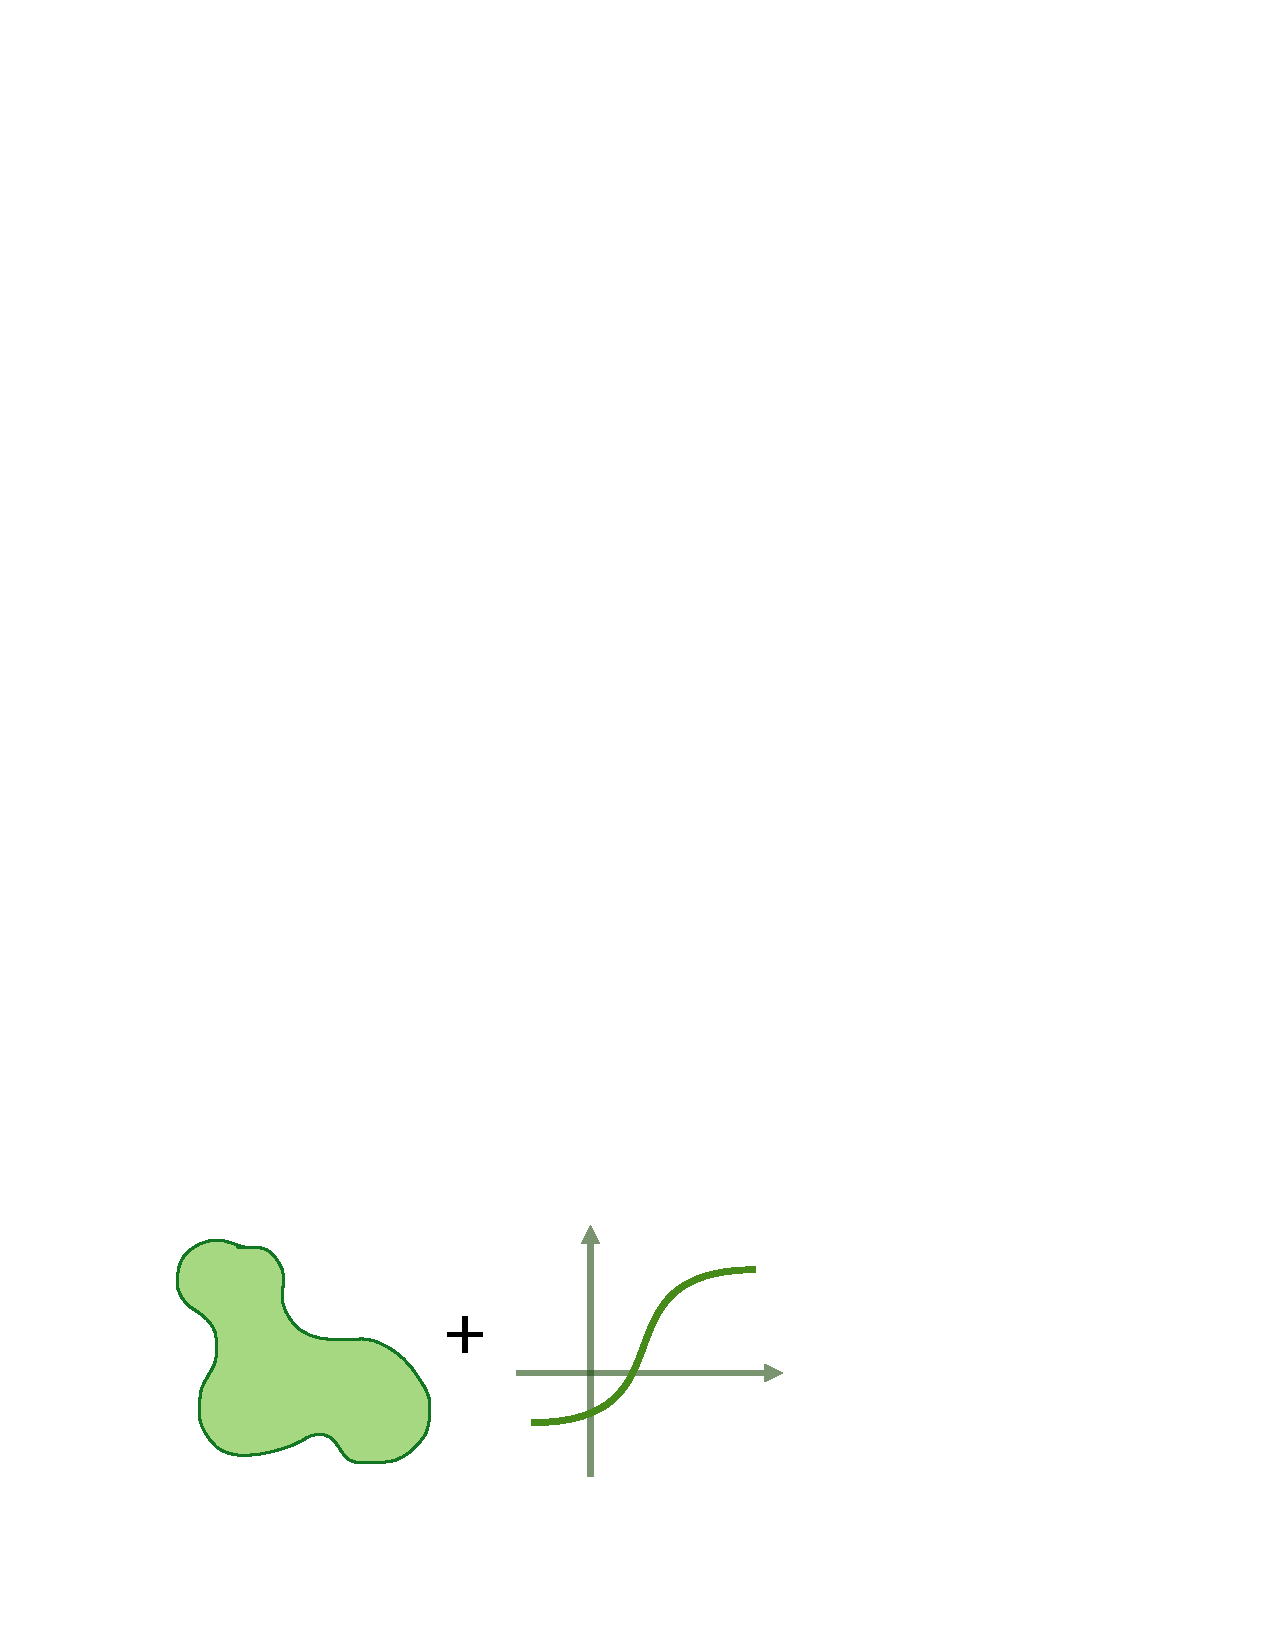
\includegraphics[width=9cm]{images/intro/objective_onegeom_onefct.pdf}};
							%		\node[color2,font=\Large] at (1.6,0.1) {+};
							%		\node at (3.5,0.8) {Several Functions};
							%		\node[draw=none, inner sep=0pt] at (3.5,0) {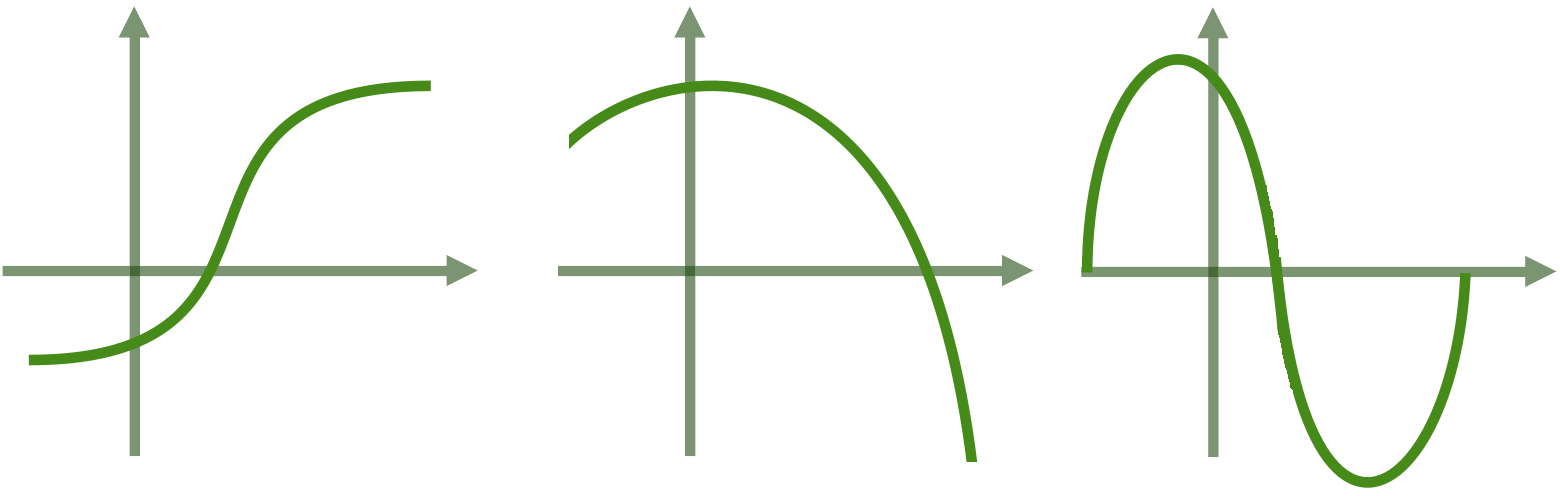
\includegraphics[width=3cm]{images/intro/objective_fct.png}};
							
							\draw[->, color2, line width=4.5pt] (6,0.3) -- (9,0.3);
							
							\node[align=center] at (13,3.8) {Get PINNs \\ prediction};
							\node[draw=none, inner sep=0pt] at (13,-0.3) {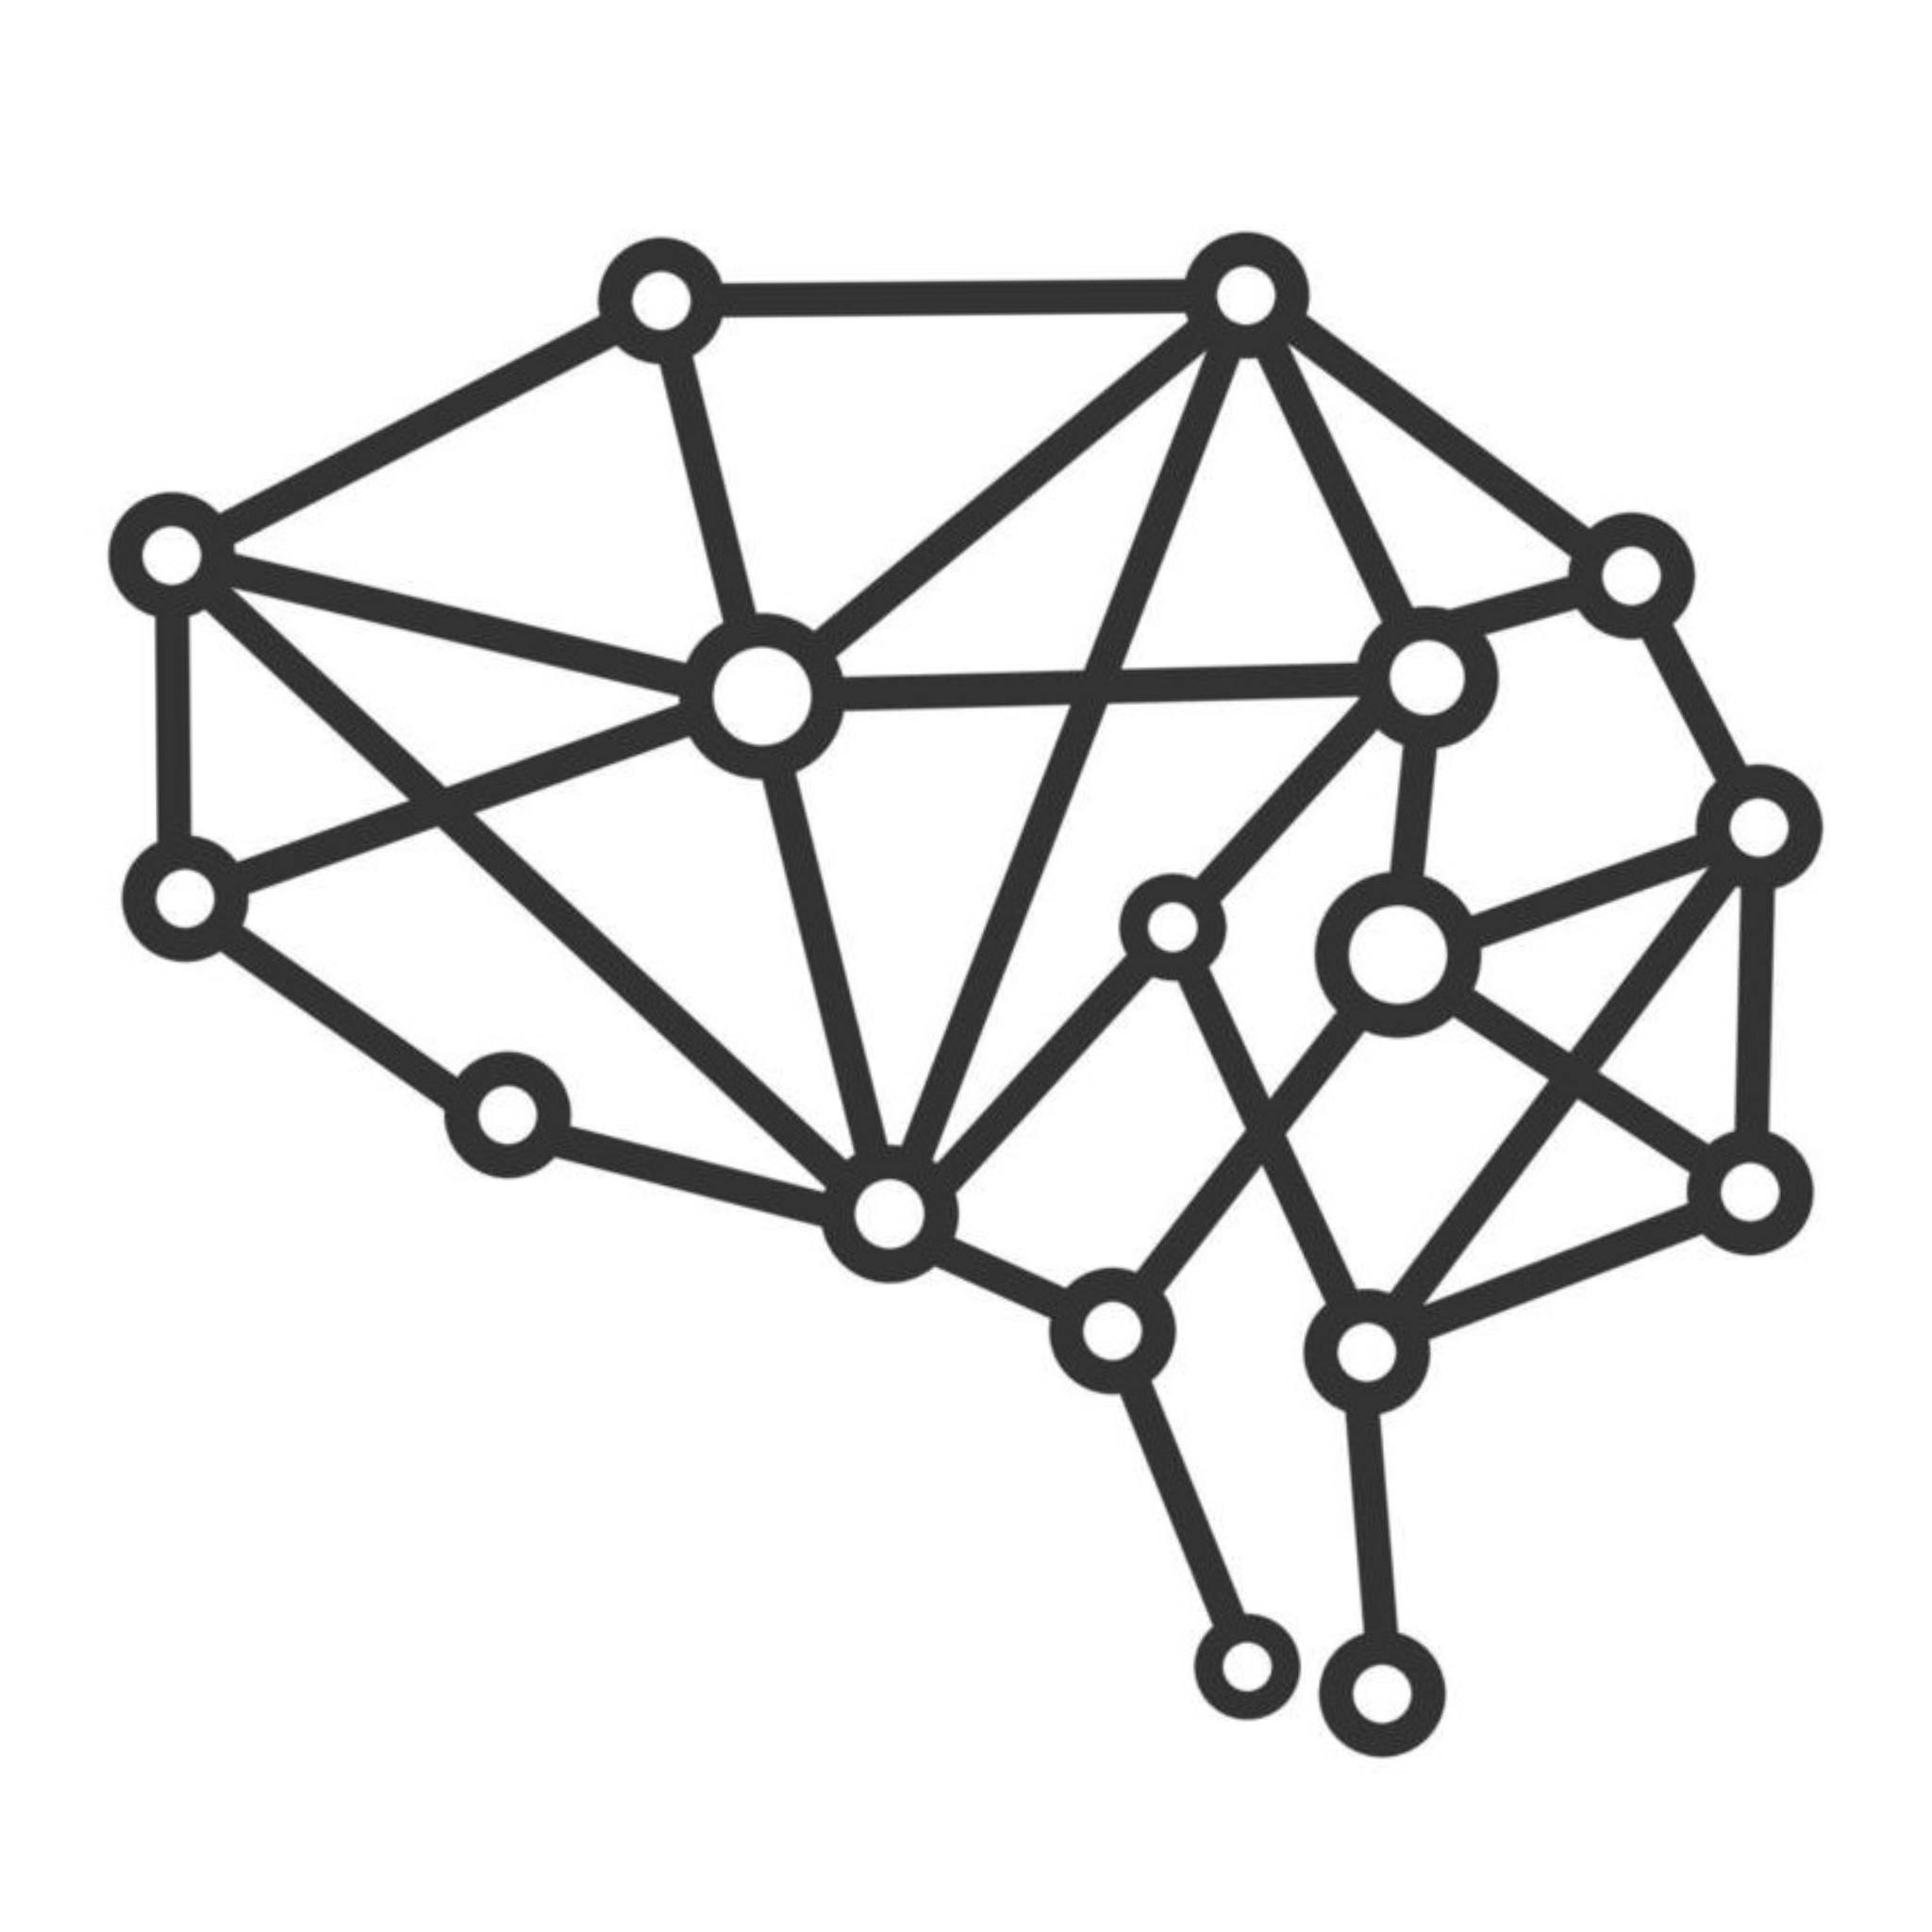
\includegraphics[width=6cm]{images/intro/objective_pinns.png}};
							
							% Ajouter une flèche entre les deux rectangles
							\draw[->, color2, line width=4.5pt] (17,0.3) -- (20,0.3);
							\draw[draw=black] (21,-3) rectangle ++(10,8.2);	
							\node[align=center] at (26,3.8) {Correct prediction \\ with FEM \cite{Ern2004TheoryAP}};
							\node[draw=none, inner sep=0pt] at (26,-0.3) {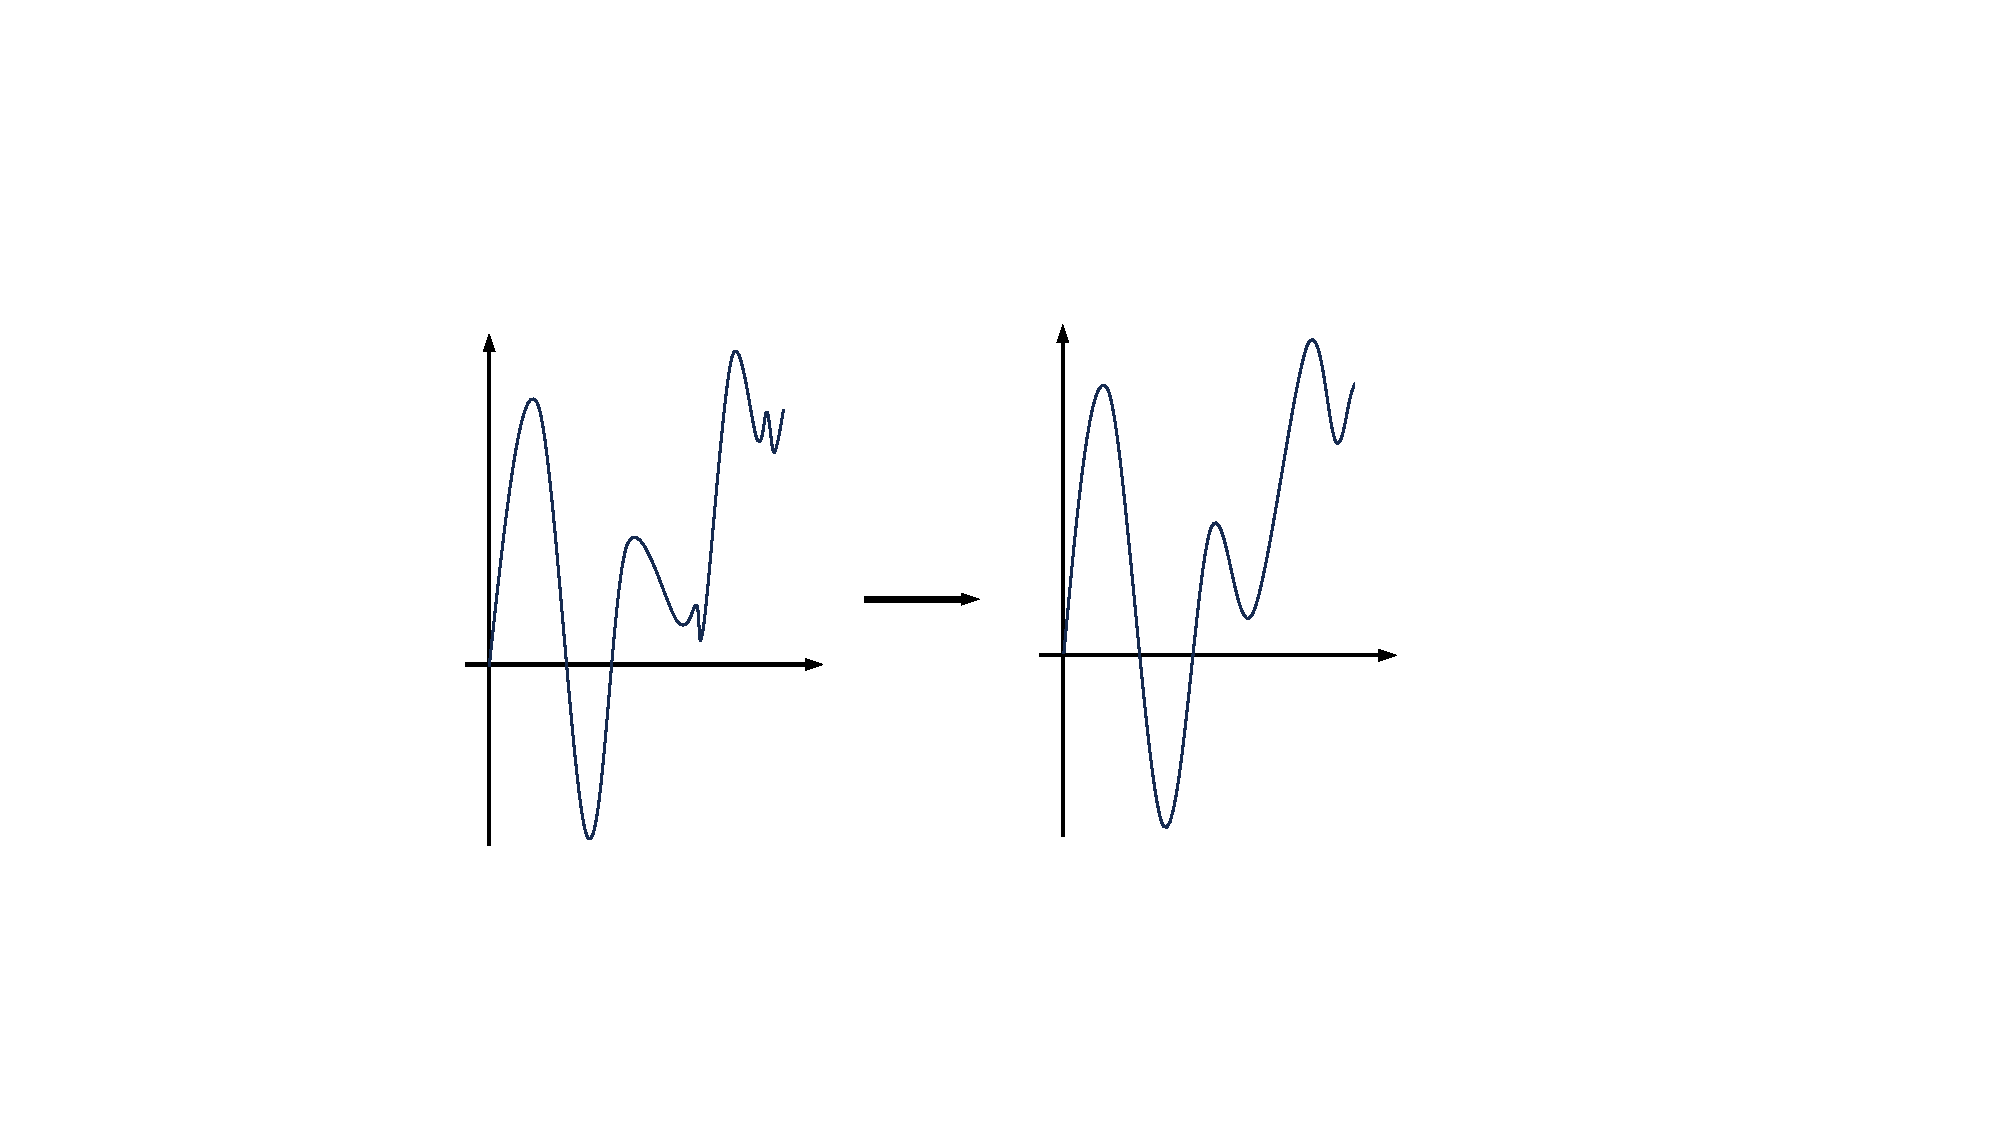
\includegraphics[width=8.5cm]{images/intro/objective_corr.pdf}};		
						\end{tikzpicture}
					\end{center}
				\end{tcolorbox}
			\end{minipage}
		\end{center}		
	
		\vspace{20pt}

		\textbf{Perspective :} Create real-time digital twins of an organ (e.g. liver).
		\vspace{-20pt}
}
		
	\node[rotate=-30,below left=0.5cm and -0.5cm] at (topright) {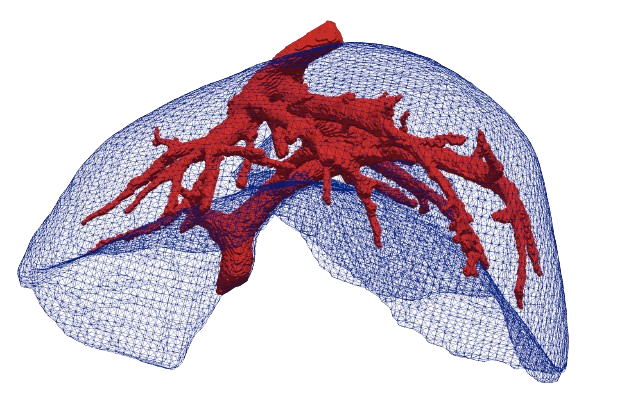
\includegraphics[width=9cm]{images/intro/foie.png}};

	% \block{Poisson problem with Dirichlet boundary conditions}{
	% 	\vspace{10pt}
		
	% 	Find $u : \Omega \rightarrow \mathbb{R}^d (d=1,2,3)$ such that
	% 	\begin{equation}
	% 		\left\{\begin{aligned}
	% 			&-\Delta u(x) = f(x) \quad \text{in } \Omega, \\
	% 			&u(x) = g(x) \quad \text{on } \Gamma
	% 		\end{aligned}\right. \label{edp} \tag{$\mathcal{P}$}
	% 	\end{equation}
	% 	with $\Delta$ the Laplace operator, $\Omega$ a smooth bounded open set and $\Gamma$ its boundary.
	% }

% 	\block{PINNs \textnormal{\large - Physics-Informed Neural Networks \cite{raissi_physics-informed_2019}}}{
% 		\begin{minipage}{0.6\linewidth}
% 			\vspace{-40pt}
% 			\textbf{Implicit neural representation.}
% 			\begin{equation*}
% 				u_\theta(x)=u_{NN}(x)
% 			\end{equation*}
% 			with $u_{NN}$ a neural network (e.g. a MLP).
% 		\end{minipage}
% 		\begin{minipage}{0.36\linewidth}
% 			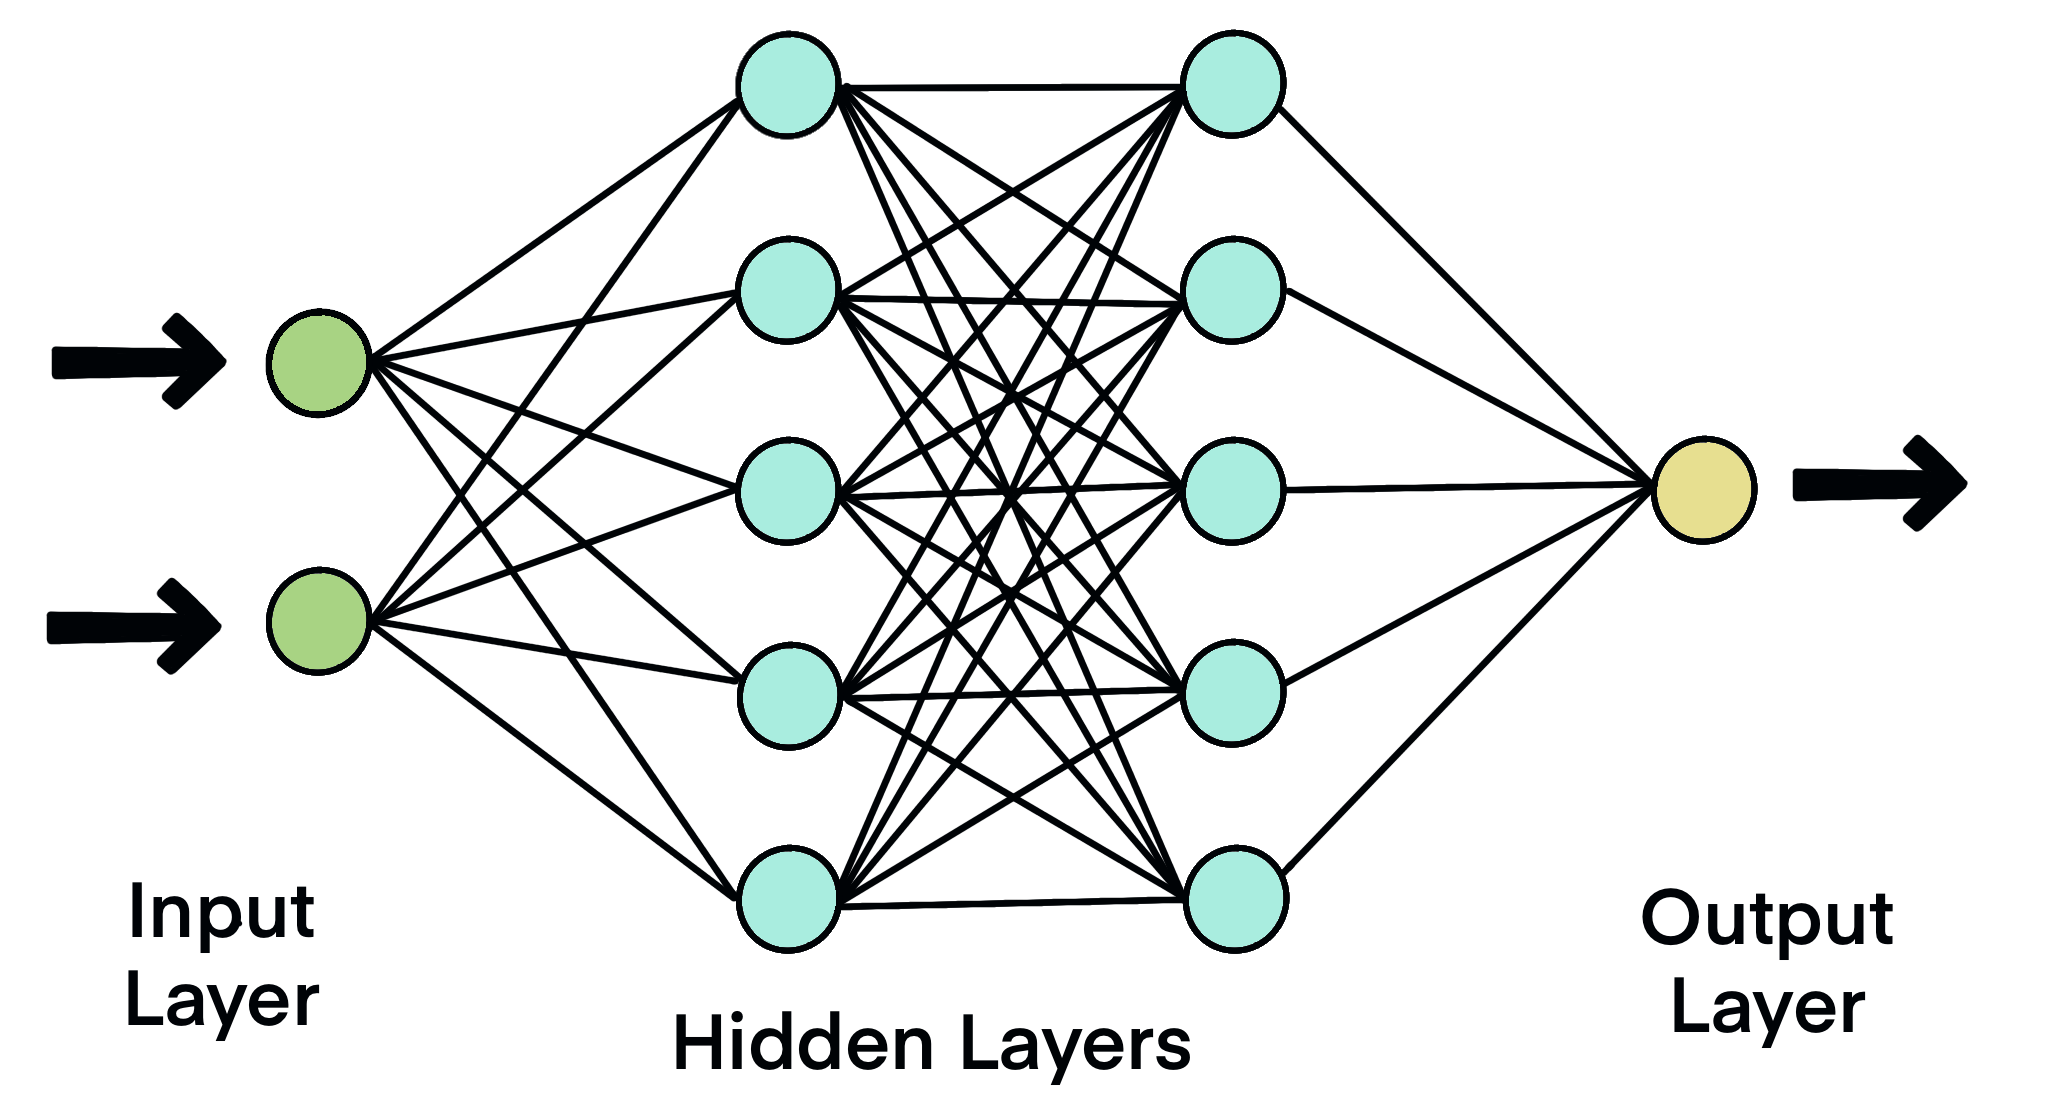
\includegraphics[width=0.85\linewidth]{images/intro/MLP_schema.png}
% 		\end{minipage}
		
% 		\vspace{-15pt}
		
% 		\textbf{DoFs Minimization Problem.}
		
% 		Considering the least-square form of (\ref{edp}), our discrete problem is
% 		\begin{equation*}
% 			\displaystyle \bar{\theta}=\argmin_{\theta\in\mathbb{R}^m} \alpha J_{\text{in}}(\theta)+\beta J_{\text{bc}}(\theta)
% 		\end{equation*}
% 		with $m$ the number of parameters of the NN and
% 		\begin{equation*}
% 			J_{\text{in}}(\theta)=\frac{1}{2}\int_\Omega (\Delta u_\theta + f)^2  \qquad \text{and} \qquad J_{\text{bc}}(\theta)=\frac{1}{2}\int_{\partial\Omega} (u_\theta-g)^2
% 		\end{equation*}	
% 	}


% 	\block{Finite Element methods}{
% 		\textbf{Variational Problem.} Let's define $V$ as a Hilbert space.
% 		\begin{equation*}
% 			\text{Find } u \in V \text{ such that, } \; \forall v\in V, \; a(u,v)=l(v)
% 		\end{equation*}
% 		with $a$ a bilinear form and $l$ a linear form defined as
% 		\begin{equation*}
% 			a(u,v)=\int_\Omega \nabla u \cdot \nabla v \quad \text{and} \quad l(v)=\int_\Omega f v.
% 		\end{equation*}
		
% 		\vspace{10pt}
		
% 		\textbf{Approach Problem.} Let's define $V_h$ as a finite-dimensional subspace of $V$ ($V_h\subset V$).
% 		\begin{equation*}
% 			\text{Find } u_h \in V \text{ such that, } \; \forall v_h\in V, \; a(u_h,v_h)=l(v_h)
% 		\end{equation*}
% 		with $u_h\in V_h$ an approximate solution of $u$ and $N_h=\dim(V_h)$.

% 		\vspace{10pt}

% 		\textbf{Linear System.} Let's define $\big\{\varphi_1,\dots,\varphi_{N_h}\big\}$ a basis of $V_h$.
% 		\begin{equation*}
% 			AU=b
% 		\end{equation*}
% 		with
% 		\begin{equation*}
% 			A=\big(a(\varphi_i,\varphi_j)\big)_{1\le i,j\le N_h}, \quad U=\big(u_i\big)_{1\le i\le N_h} \quad \text{and} \quad b=\big(l(\varphi_j)\big)_{1\le j\le N_h}
% 		\end{equation*}
% 	}

% 	\node[below left=1cm and 1cm] at (topright) {
\includegraphics[width=6cm]{images/intro/mesh.png}};

